\chapter{Beam Backgrounds}
\label{chap:beamBack}

	As electrons and positrons circle the HER and LER, some of them are lost from the beam as they collide with the residual gas in the beampipe and with other beam particles. These collisions move the particles out of a stable orbit, causing them to collide with the beampipe and other nearby materials, causing showers of particles. This chapter discusses some of the ways that particles can be lost from the beam and some of the effects of that loss.


\section{Beam-Gas Interactions}
\label{sec:beamGas}

\begin{figure}[htb]
	\centerfloat
		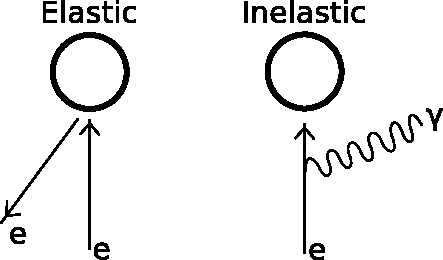
\includegraphics{images/beambeamCartoon}
	\caption[Beam-gas scattering]{Beam-gas scattering.}		
	\label{fig:BGasScat}
\end{figure}


\subsection{Elastic collisions}

	The beampipe is designed to operate under a vacuum of 10~nTorr and as such there are still residual gas atoms in the beampipe. When a beam particle collides with an atom of residual gas in the beampipe, the collision is elastic and there is very little kinetic energy transferred to the gas atom. The beam particle, however, undergoes a large scattering, which can send it outside the acceptance of the beam orbit. The cross section for this interaction is given by \cite{moller1999beam, Marin:1999ss}:
\begin{equation}
	{\sigma_{\mathrm{scatt}}=\frac{2\pi r_eZ^2}{\gamma^2}\frac{\beta_1\beta_2}{d^2}}
	\label{eqn:coulomb}
\end{equation}
where $r_{e}$ is the classical electron radius, $\gamma$ is the relativistic Lorentz factor, $Z$ is the atomic number of the target nucleus, $\beta_1$ and $\beta_2$ are the betatron functions, and $d$ is the size of beam aperture.


\subsection{Inelastic collisions}
\label{sec:brem}

	Beam particles emit bremsstrahlung radiation as they interact with the residual gas atoms in the beampipe. If the energy lost to the bremsstrahlung photon is high, the particle that emitted it will fall out of the momentum acceptance of the ring. The cross section for bremsstrahlung of electrons on atomic nuclei is given by \cite{moller1999beam, Marin:1999ss}:
\begin{equation}
	{\sigma_{\mathrm{brems}}=\frac{16r_e^2Z^2}{411}\ln\left [ \frac{183}{Z^{1/3}} \right ]\ln\left [ \frac{E}{\varepsilon _{RF}}-\frac{5}{8} \right ]}
	\label{eqn:brems}
\end{equation} 
where $r_e$ is the classical electron radius, $Z$ is the atomic number of the target nucleus, $\varepsilon _{RF}$ is the energy acceptance, and $E$ is the beam energy.

\subsection{Beam-Gas Beam Loss}

	The beam loss due to beam-gas effects is given by \cite{moller1999beam, malyshev2012gas}:
\begin{equation}
	{-\frac{1}{I}\frac{dI}{dt}=\frac{1}{\tau_{\mathrm{gas}}} = v\sum \sigma_{i} n_{i}}
\end{equation}
where $\tau_{\mathrm{gas}}$ is the beam lifetime from the beam-gas effects, $I$ is the beam current, $v$ is the velocity of the beam particles, $\sigma_{i}$ is the beam-gas cross section for each gas species, and $n_i$ is the atomic density of each species. If the gas mixture is constant, this can be rearranged to:
\begin{equation}
	{\frac{dI}{dt}\propto - I P}
	\label{eqn:simpleBeamGas}
\end{equation}
where $P$ is the beampipe pressure, which is proportional to the density of the gas.

If the gas mixture is changing, this change must be accounted for. Both the elastic and inelastic cross sections depend on $Z^2$. This modifies Eqn \ref{eqn:simpleBeamGas} to be:
\begin{equation}
	{\frac{dI}{dt}\propto  - I P Z^{2}}
	\label{eqn:complexBeamGas}
\end{equation}
which ignores the $\ln(183/Z^{1/3})$ term in Eqn \ref{eqn:brems}, but this term is roughly constant for $2>Z>12$.

\section{Beam-Beam Interactions}

\subsection{Touschek effect}

\begin{figure}[htb]
	\centerfloat
		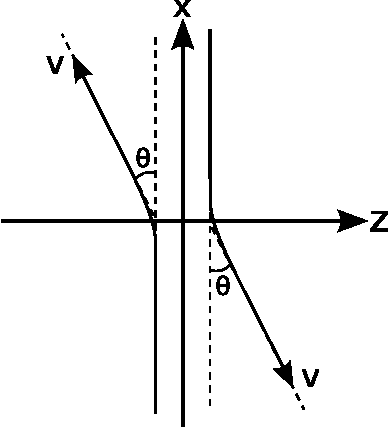
\includegraphics[scale=0.8]{images/TouschekScatter}
	\caption[Touschek scattering in the centre of mass of the bunch]{Touschek scattering in the centre of mass of the bunch. Momentum is transferred from the $x$-direction (transverse) to the $z$-direction (longitudinal). In this figure, the bunch is travelling in the $z$ direction \cite{Wolski}.}
	\label{fig:TousScat}
\end{figure}

	The Touschek effect is a scattering effect that occurs between particles in the same bunch. Particles in a bunch undergo large angle Coulomb collisions, which transfers momentum to the longitudinal plane. This can force particles out of the momentum acceptance of the ring, causing the particles to be lost. Touschek lifetime, $\tau_{T}$, is given by:
\begin{equation}
	{\frac{1}{\tau_{T}} = -\frac{1}{N_{b}}\frac{dN_{b}}{dt} \propto -\frac{N_{b}}{\sigma_{y}}}
	\label{eqn:touschekEqn}
\end{equation}
where $N_{b}$ is the number of particles in a bunch, $\sigma_{y}$ is the vertical beam size, and $dN_{b}/dt$ is the loss rate of the beam \cite{Wolski}. As shown in Table~\ref{tab:SKBBEAM}, the horizontal beam size is much larger than the vertical beam size, and as such it remains roughly constant. During the machine studies, the number of particles in a beam was not measured, but the number of bunches in the whole ring was. This can be related to the number of particles in each bunch using the relationship:
\begin{equation}
	{N_{b} \propto\frac{I}{N_{\mathrm{Bunch}}}}
\end{equation}
where $N_{\mathrm{Bunch}}$ is the number of bunches in the entire ring, and $I$ is the beam current. Substituting this into Eqn \ref{eqn:touschekEqn} gives:
\begin{equation}
	{\frac{dI}{dt}\propto-\frac{I^2}{N_{\mathrm{Bunch}}\sigma_{y}}}
\end{equation}


%\section{Other interactions}

%collision with dust

%electron cloud effect

\section{Radiative Bhabhas}

Radiative Bhabhas (RBB) occur when an electron and positron scatter off each other, with one or both particles emitting a photon. This photon can cause showers of electrons and photons in the detector. For low angle scattering, some particles will be knocked out of stable orbit and can be scattered into the detector, producing more showers. These showers can lead to degradation in the performance of the detector. This was not an issue in Phase~I of BEAST~II since there were no collisions.

\section{Neutron Production}

%	It is not immediately obvious how the neutrons that the \he tubes will measure are produced, since SuperKEKB is an \epem accelerator, and neutrons are hadrons. 


The neutrons that the \he tubes measured are produced by bremsstrahlung photons (note that this refers not only to the bremsstrahlung discussed in \S~\ref{sec:brem}, but also to bremsstrahlung of electrons interacting with other materials near the beam, such as the beampipe) producing photo nuclear reactions. Beam-gas, Touschek, and RBB events cause electrons to be knocked out of stable orbits, which leads to collisions with the beampipe walls, producing the bremsstrahlung photons that then produce neutrons. These neutrons are produced with a large energy distribution, with a threshold between 4 and 20 MeV. As these neutrons travel through various materials, they become thermalized \cite{PDGBook}.




% There is a process called the giant dipole resonance that is responsible for producing neutrons in \epem accelerators. A photon's electric field collectively excites the nucleus of an atom (in the beampipe, or any other structure nearby), causing the protons and neutrons in the nucleus to oscillate. This oscillation is quickly damped by friction. 







































